\begin{enumerate}[label=\thesection.\arabic*.,ref=\thesection.\theenumi]
\numberwithin{equation}{enumi}
\item Using Nyquist criterion find the range of $K$ for which closed loop system is stable.
\begin{align}
    G(s) &= \frac{K}{s(s+6)}. 
    \label{eq:ee18btech11028_1_1}
\\
    H(s) &= \frac{1}{s+9}
    \label{eq:ee18btech11028_1_2}
\end{align}

\solution
The system flow can be described as,

\begin{figure}[!ht]
    \begin{center}
        \resizebox{\columnwidth}{!}{%\begin{figure}
\tikzstyle{block} = [draw, fill=blue!20, rectangle, 
        minimum height=1cm, minimum width=1cm]
    \tikzstyle{sum} = [draw, fill=blue!20, circle, node distance=1cm]
    \tikzstyle{input} = [coordinate]
    \tikzstyle{output} = [coordinate]
    \tikzstyle{pinstyle} = [pin edge={to-,thin,black}]
    
    % The block diagram code is probably more verbose than necessary
    \begin{tikzpicture}[auto, node distance=2cm,>=latex']
        % We start by placing the blocks
        \node [input, name=input] {X(s)};
        \node [sum, right of=input] (sum) {};
        \node [block, right of=sum] (controller) {$\frac{1}{s(s+6)}$};
        \node [block, right of=controller] (system) {$K$};
        % We draw an edge between the controller and system block to 
        % calculate the coordinate u. We need it to place the measurement block. 
        \draw [->] (controller) -- node[name=u] {} (system);
        \node [output, right of=system] (output) {};
        \node [block, below of=u] (measurements) {H(s)};
    
        % Once the nodes are placed, connecting them is easy. 
        \draw [draw,->] (input) -- node {$X(s)$} (sum);
        \draw [->] (sum) -- node {} (controller);
        \draw [->] (system) -- node [name=y] {$Y(s)$}(output);
        \draw [->] (y) |- (measurements);
        \draw [->] (measurements) -| node[pos=0.99] {$-$} 
            node [near end] {} (sum);
    \end{tikzpicture}
%\end{figure}
}
    \end{center}
    \caption{}  
    \label{fig:ee18btech11028_1_fig1}
\end{figure}


\begin{align}
    G_{1}(s) = \frac{1}{s(s+6)}. 
    \label{eq:ee18btech11028_1_3}
\end{align}

For Nyquist plot, 

\begin{align}
    \text{Im} \cbrak{G_{1}(\j \omega)H(\j \omega)} &= \frac{-(54 - \omega^{2})}{(\omega)(\omega^{2}+56)(\omega^{2} + 81)}
    \label{eq:ee18btech11028_1_5}
\\
    \text{Re} \cbrak{G_{1}(\j \omega)H(\j \omega)} &= \frac{-15 \omega}{(\omega)(\omega^{2}+56)(\omega^{2} + 81)}
    \label{eq:ee18btech11028_1_4}
\end{align}

From \eqref{eq:ee18btech11028_1_5} and \eqref{eq:ee18btech11028_1_4}

\begin{figure}[!h]
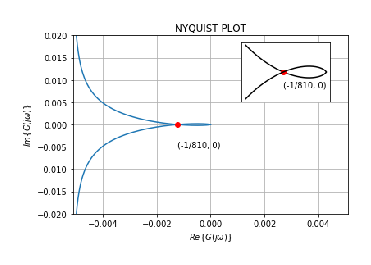
\includegraphics[width=\columnwidth]{./figs/ee18btech11028/ee18btech11028_1.eps}
    \centering
  \caption{Nyquist plot for $G_{1}(s)H(s)$}
  \label{fig:ee18btech11028_1_fig2}
\end{figure}


\textbf{Nyquist Stability Criterion:}
\begin{align}
    N = Z - P
\end{align}

where Z is \# unstable poles of closed loop transfer function, P is \# unstable poles of open loop transfer function
and N is \# clockwise encirclement of \brak{-1/K,0}.

For stable system, 
\begin{align}
    Z = 0
\end{align}

From \eqref{eq:ee18btech11028_1_2} and \eqref{eq:ee18btech11028_1_3},
\begin{align}
    P = 0
\\
    \implies N = 0
    \label{eq:ee18btech11028_1_7}
\end{align}




Since, there is a zero at origin, an infinite radius half circle will enclose the right hand side of end points of the Nyquist plot.
So for \eqref{eq:ee18btech11028_1_7},
\begin{align}
    \implies \frac{-1}{K} < \frac{-1}{810}
    \implies K < 810
\end{align}

And also,

\begin{align}
    K > 0
\\
    \implies 0 < K < 810     
\end{align}


The following python code generates  Fig. \ref{fig:ee18btech11028_1_fig2}
\begin{lstlisting}
    codes/ee18btech11028_1.py
\end{lstlisting}
\end{enumerate}